\documentclass[12pt,a4paper]{article}
\usepackage{latexsym}
\usepackage{amsfonts}
\usepackage{enumitem}
\usepackage{multicol}
\usepackage{amsmath}
\usepackage{amssymb}
\usepackage{geometry}
\usepackage[english]{babel}
\usepackage[latin1]{inputenc}
\usepackage[T1]{fontenc} %inclue les charact?res dans le pdf
\usepackage{graphicx}
\usepackage{epsfig}
\usepackage{url}
\usepackage[verbose, bookmarksopen=false, hypertexnames=false,linktocpage,bookmarksnumbered,colorlinks]{hyperref}
\usepackage{lineno}
\usepackage{listings}
\usepackage{hyperref}
\hypersetup
{
    colorlinks  = true,
    citecolor   = blue,
    linkcolor   = black
}

\usepackage{afterpage}
\newcommand\blankpage{
    \null
    \thispagestyle{empty}
    %\addtocounter{page}{-1}
    \newpage}

\usepackage[justification=centering]{caption}
\usepackage{float}
\usepackage{titlesec}
\setcounter{secnumdepth}{4}
\setcounter{tocdepth}{4} %for table of content
\titleformat{\paragraph}
{\normalfont\normalsize\bfseries}{\theparagraph}{1em}{}
\titlespacing*{\paragraph}
{0pt}{3.25ex plus 1ex minus .2ex}{1.5ex plus .2ex}

\usepackage{fancyhdr}    
\fancyhf{}
\pagestyle{fancy}
\setlength{\headheight}{15pt}

\fancyheadoffset{0.1\textwidth}
\fancyfootoffset{0.1\textwidth}
\setlength{\footskip}{40pt}
\lhead{\slshape \rightmark}    
\rhead{\slshape \hyperlink{toc}{\leftmark}}
\rfoot{\thepage}
\lfoot{Semester Project MA-1 | Cyril Schmitt - LASA - IMT - EPFL}
\renewcommand{\footrulewidth}{0.4pt}

%Titlepage
\thispagestyle{plain}
\title{Semester project}
\author{Cyril Schmitt}

\geometry{ hmargin=2.5cm, vmargin=2.5cm }

\renewcommand{\maketitle}{
\begin{titlepage}
\centering

\includegraphics[width=5cm]{img/EPFL_LOGO.eps}\\
\vspace*{3cm}
\LARGE{\textbf{Simplifying user/robot interface by  \linebreak using speech commands
\\}}
Semester project
%TODO : title to check again after\\

\vspace*{2cm}
\Large{Cyril Schmitt} \\
\vspace*{2cm}
\normalsize{\'{E}cole Polytechnique F\'{e}d\'{e}rale de Lausanne\\Learning Algorithms and Systems Laboratory\\}
\vspace*{1cm}
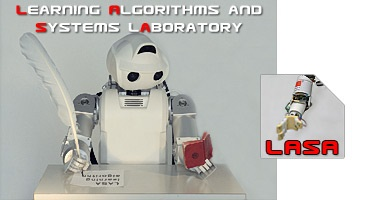
\includegraphics[width=7cm]{img/lasa-logo.jpeg}\\
\vspace*{2cm}
\large{Supervised by Felix Duvallet, Klas Kronander and Professor Aude Billard\\}
\vspace*{1cm}
\today
\end{titlepage}
}

%###########################################################################
\begin{document}
% -------------- title
\maketitle
\thispagestyle{plain}

% -------------- blankpage
\blankpage

% -------------- abstract
\begin{abstract}
This project is aiming to simplify the interface between user and robots by using speech. This functionality will allows the user to change the speed of the robot, give a command to execute and teach new commands.

In order to develop this project we mainly used Python for coding and ROS to communicate between each node of the project. The major component of the project is the state machine which will create the path the program will follow to create the dialogue between the user and the robot.

Some experiments have been made including the one to select the best keywords the program will have to recognize to do what the user want the robot to do or the final experiment of the program to get feedbacks from users.

These experiments provided several insight for future improvement of the dialogue system.\\
\\
\underline{Catch phrase:} Implementing Dialogue using a State Machine is an adaptable, robust and easy way to interact with robots

\end{abstract}
\clearpage

% ------------- table of content
\newpage
\thispagestyle{empty}
\begin{tableofcontents}
\addtocontents{toc}{\protect\hypertarget{toc}{}}
\end{tableofcontents}


%\thispagenumber{1}
\clearpage
\section{Introduction}
\subsection{Motivation}
Todays engineer are developing complex robots to do some incredible tasks, it also involves the difficulty to control such robots. In fact the harder the task is the more probable the controller also is. We also know that engineer are expensive to a company regarding to a regular employee and also that they are over-qualified to just control the robot they developed.

Taking all these aspects into account, we aimed to develop a way to control robots in an easier way. In fact the goal was to be able to teach some commands to a robot by using speech. The interest of such a development is that it will allow any user to use industrial and complex robots by using vocal commands. This document explains how this program has been developed.

\subsection{Objectives}

We can classify the objectives into two parts. The first will be the main goals and then the secondary goals.\\
\\Main goals:
\begin{itemize}
  \item Controlling robot using speech
  \item Teaching command to a robot using speech
\end{itemize}
Secondary goals:
\begin{itemize}
  \item Adaptability of the code to all robots
  \item Facility of use without instructions
\end{itemize}

\subsection{Specifications}
\hfill \linebreak
The main specifications of the project are listed just below. Those specifications define the project itself and served as a guideline throughout the whole development: 
\begin{itemize}
  \item The user should be able to change the speed of the robot 
  \item The user should be able to give a command to the robot 
  \item The user should be able to teach a command to the robot
  \item The user should be able to control the robot just by using speech 
  \item The user should feel confident using the robot without preliminary explanation 
  \item The code should be re-usable on every other robots 
\end{itemize}

\subsection{Scenarios}
This section will let you see one scenario for each functions the program should be able to do:
\begin{figure}
\begin{center}
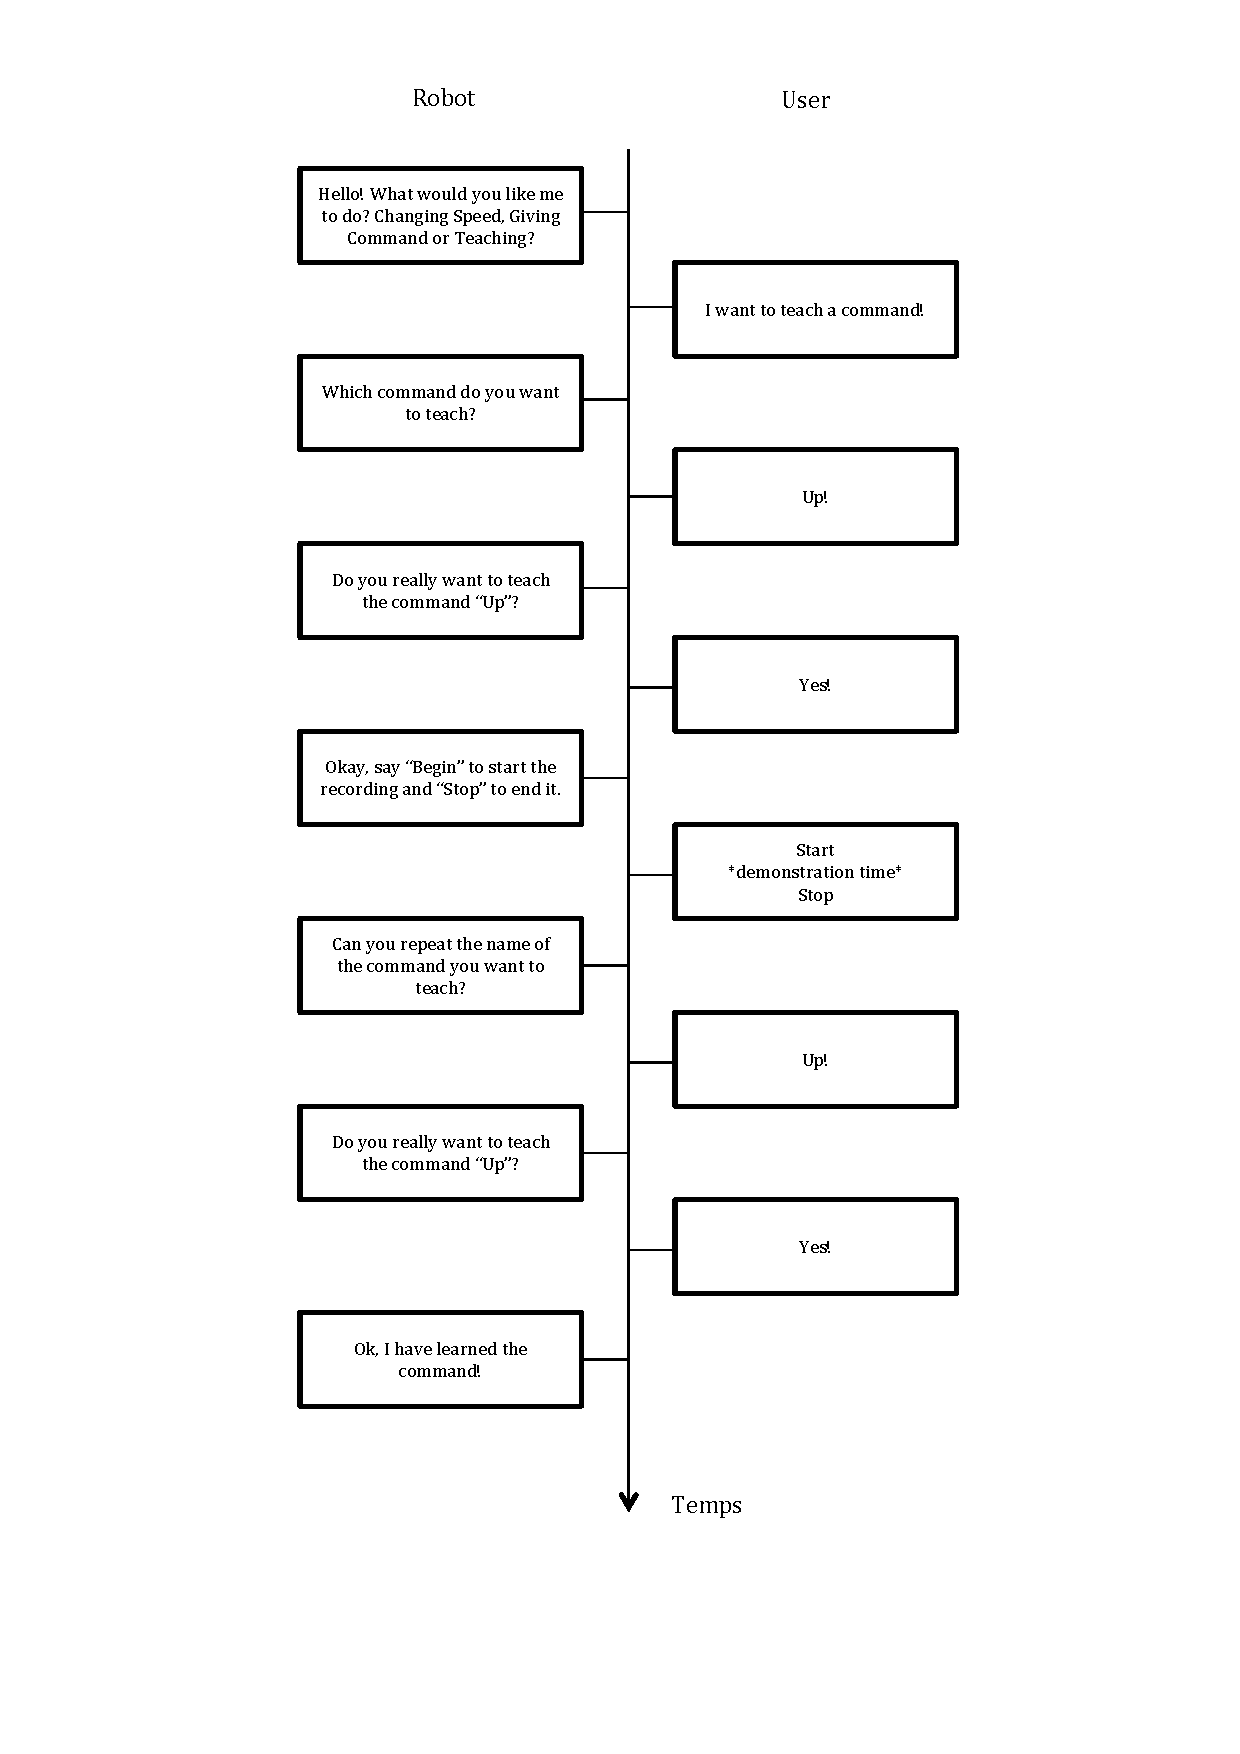
\includegraphics[width=16cm]{img/Schema_Dialogue_TeachingBranch.pdf}\\
\caption{Teaching Command Branch}
\end{center}
\end{figure}

\begin{figure}
\begin{center}
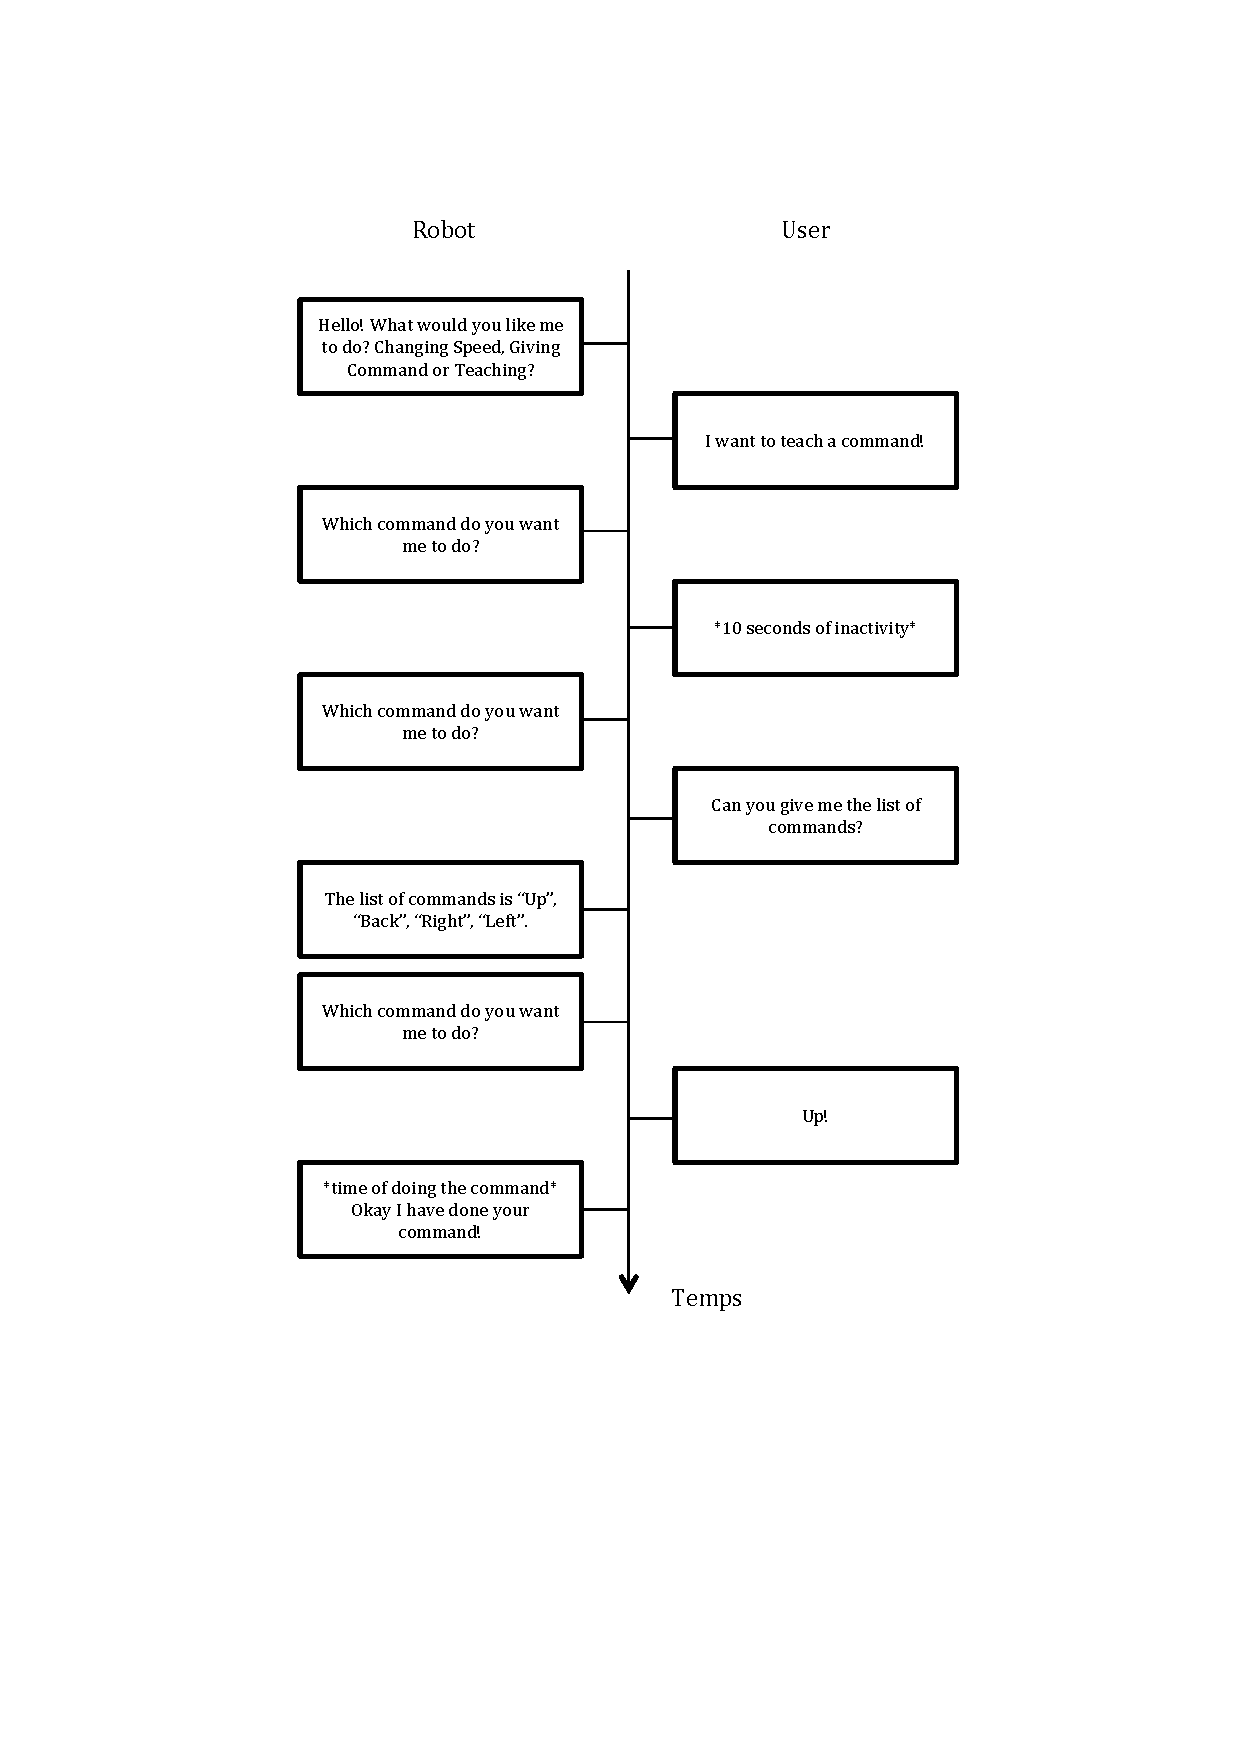
\includegraphics[width=16cm]{img/Schema_Dialogue_CommandingBranch.pdf}\\
\caption{Giving Command Branch}
\end{center}
\end{figure}

\begin{figure}
\begin{center}
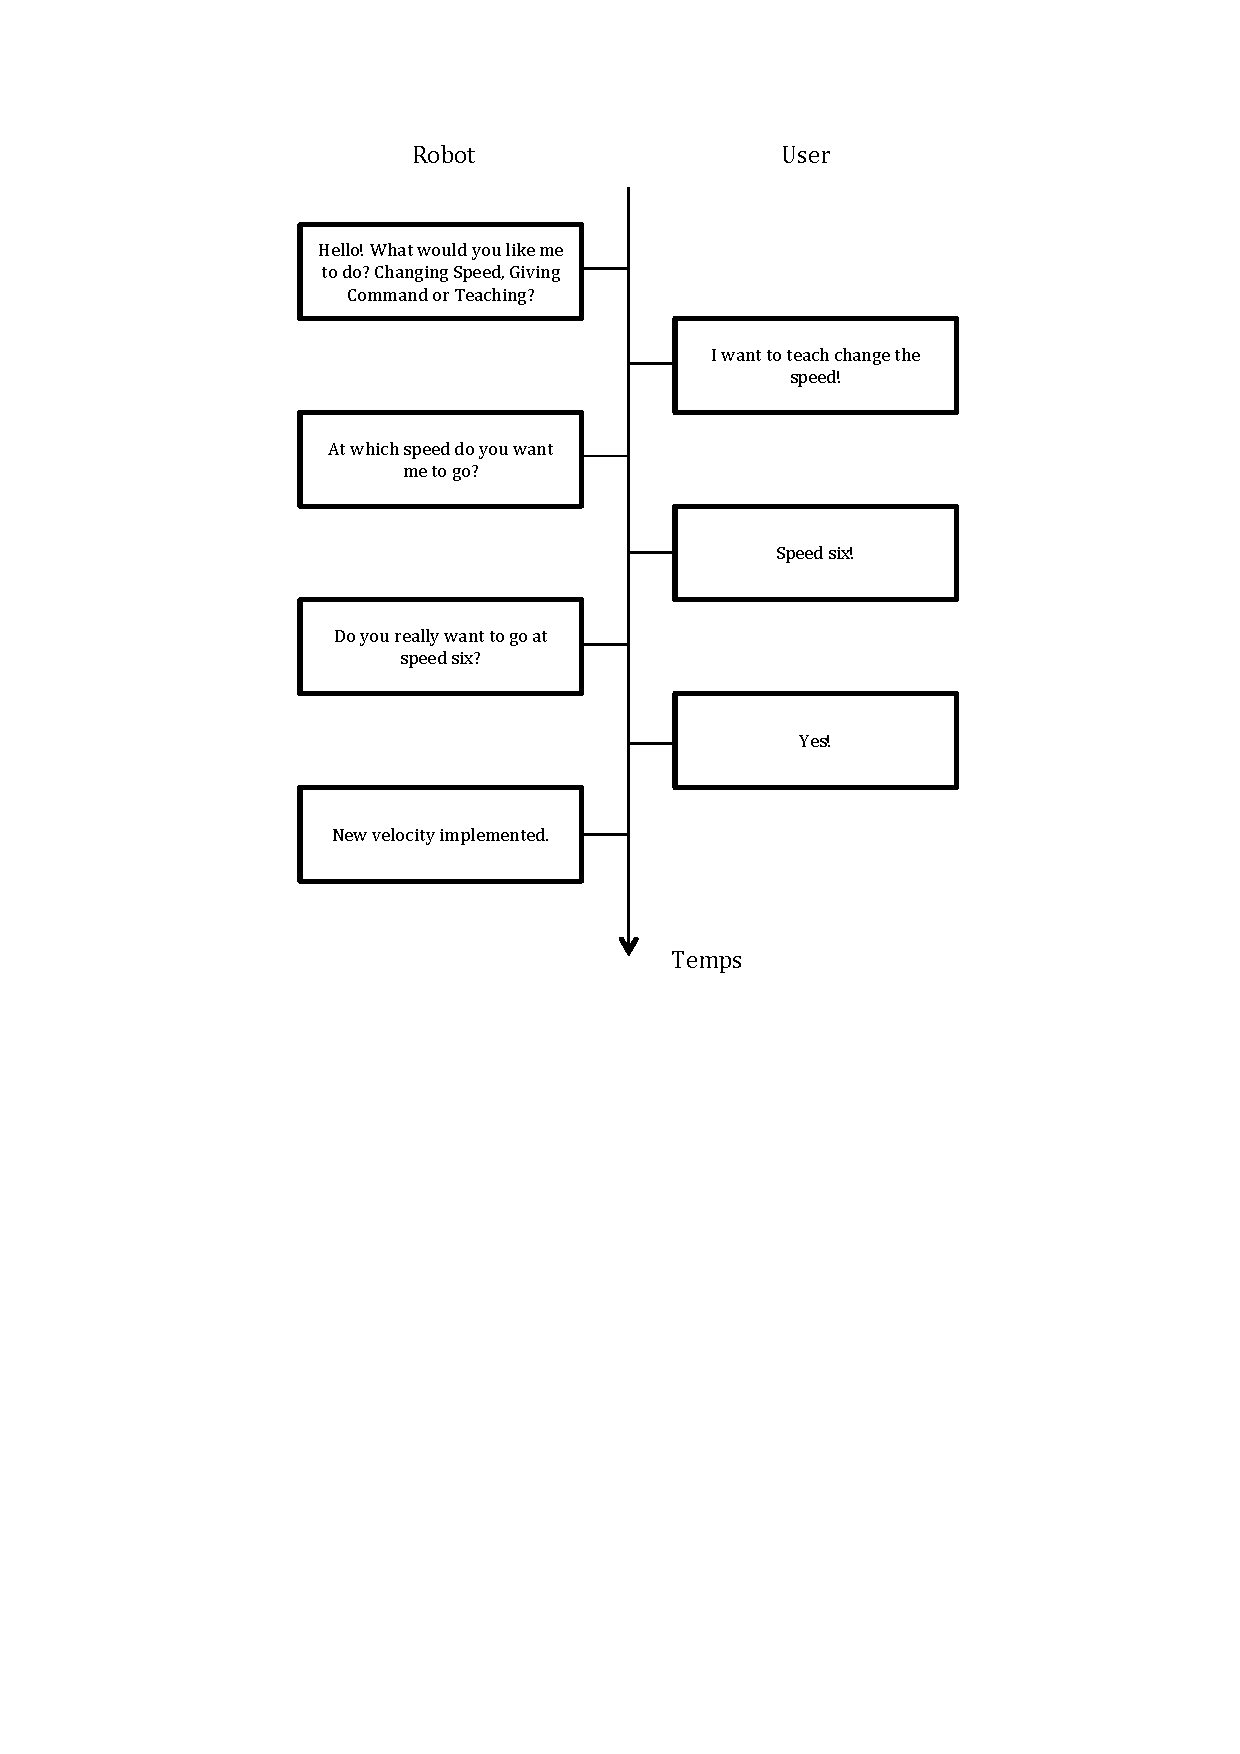
\includegraphics[width=16cm]{img/Schema_Dialogue_SpeedingBranch.pdf}\\
\caption{Changing Speed Branch}
\end{center}
\end{figure}
\clearpage
\section{Development}
\subsection{Development Methodology and Learning}

We used two development tools, the first one is Python and the second one is ROS. 

ROS is in charge here of the communication between each part of the program, and we call each part of it: node. It is by this way that information is passed one node to another. We call this information: topic. 

Python was used to develop each node of the program in order to make them do what was needed.

In order to go further into the project we develop the general structure of the program with the different functions the robot should be able to do. In order to improve the project we decided to use robot feedback, and ideally speech feedback in order to create a dialogue between the user and the robot. So we used the client sound\_play. This client can reproduce the sound of the sentence we gave it in argument. My first step for learning was to develop a small program talking back.

In order to structure the code and to lightweight it the more we can and also to make it easier to read we decided to use a state machine. In fact the structure of a state machine allows us to assembly and reuse part of the code easily as if we were imbricating one state after another. We could have also developed the code without state machine, but it would have been more difficult and annoying to develop.

Regarding the structure of the project we decided to develop State Machine by State Machine beginning with the Kernel Machine, the one that will be at the centre of the program. Once done we just had to complete this machine with machine within (see Figure 4: Schema of the program).

 \begin{figure}
 \center
 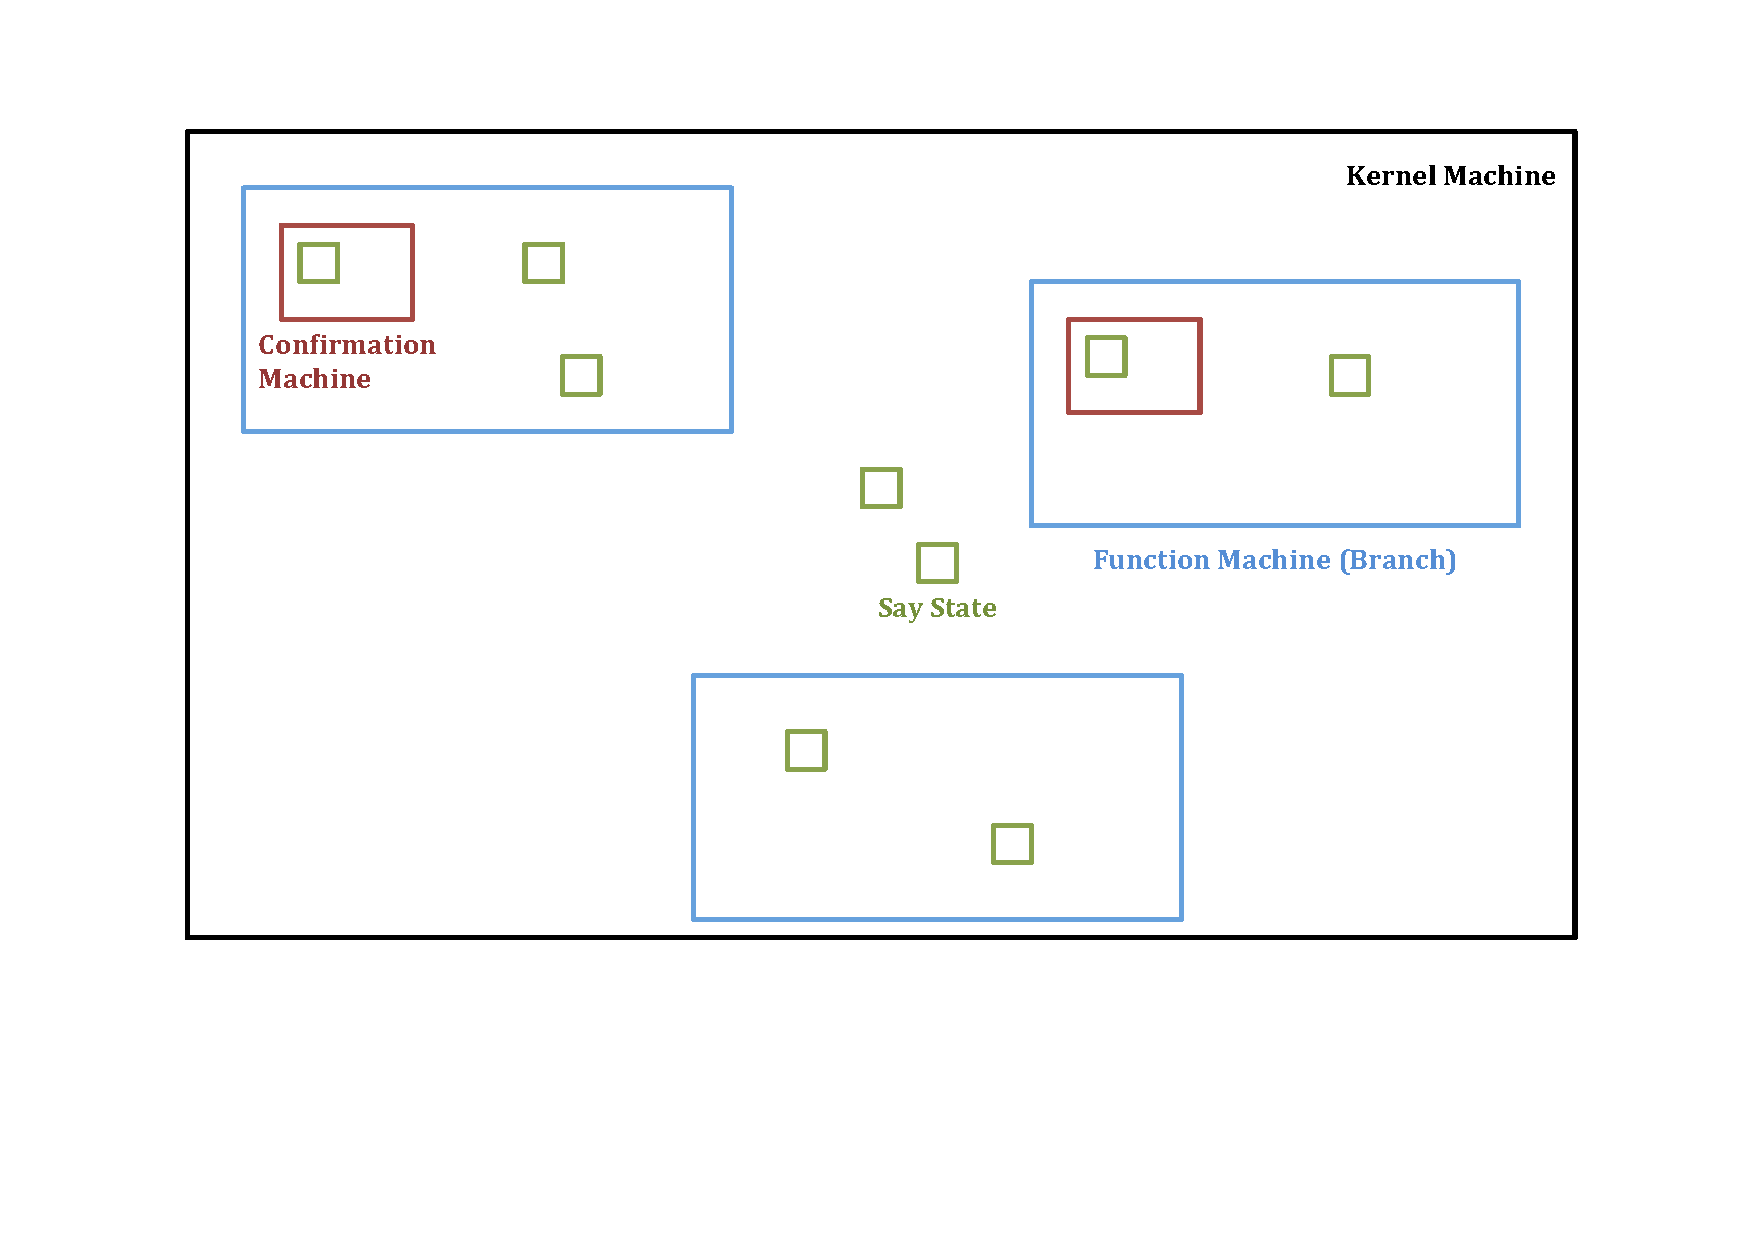
\includegraphics[width=15cm]{img/SimplificationMachineProgram.pdf}
 \caption{Schema of the program}
 \end{figure}

As seen on the Specifications we considered three branches (changing speed, giving command and teaching command) that we developed and structured with the same process for each of them. First part was to develop one branch, state by state by continuously testing the code. Once all the branches were developed, we tested it all together and took the place of a random user to see which improvement can be made to make the experience even easier. Finally small modifications were added. This process was repeated the three times for each branch. It also happened to come back to branches already developed to make some new changes after realizing some changes could be made to make it easier to use.

In parallel to the development of the state machine we used the testing of some functions using unit tests, which is a simple way to test quickly a function.

\subsection{Program Architecture}
The architecture of the program is mainly composed of a speech-to-text algorithm, a state machine, a robot interface, a robot and some development tools. In order to understand well the architecture of the program we will use the tool rqt\_graph which shows all the nodes and topics that are part of the project (see Figure 5).\\
\\
For the understanding of the lecture of the diagram:
\begin{itemize}
  \item Square shapes are representing Nodes
  \item Arrow  shapes are representing Topics
\end{itemize} \hfill \linebreak
For the understanding of the terms "publishing" and "subscribing":
\begin{itemize}
  \item "recognizer" is publishing into "state\_machine"
  \item "recognizer" is subscribing to "microphone\_capture"
\end{itemize}\hfill \linebreak
The algorithm Pocketsphinx ("Recognizer" on Figure 5) is the \underline{speech-to-text algorithm}. The node "recognizer" is subscribing to the microphone of the computer \linebreak ("microphone\_capture") and publishing into the State Machine ("state\_machine") to give text (string) corresponding to the audio we received in input in the microphone. This part is an essential part to develop a dialogue.

Since a \underline{dialogue} would not be possible with a one way communication we needed to use a robot speech feedback. This is the reason why we added the "sound\_play" client into the program. This node allows the robot to create sound and in particularly to talk and pronounce the sentence we give it into arguments. 

The State Machine will create the \underline{dialogue structure} which will be exploited to control the robot. This machine is in the middle of the project as we can easily see in the Figure 5. Three main branches are created into this State Machine which represents the three main functionalities: changing speed, giving command and teaching command. 

This State Machine will publish into the robot converter ("robot\_receiver") which is also called the \underline{robot interface}. This converter will subscribe to the State Machine. The State Machine will give to the converter some string, via the topics, that the converter will interpret. Thanks to this interface our program allows us to use the project on every robot by the simple change of the converter, in fact the only thing to change is the topic getting out of the converter which should match to the robot type we want to use. Since the State Machine is separated by the converter to the robot we can call this interface a \underline{robot-agnostic interface}.\hfill \linebreak
\\
As a fact we used the same program with the Turtlesim simulator and the Kuka.\hfill \linebreak
\\
Finally some very useful tools were used during the development but could also be used as an user/robot interface: 
\begin{itemize}
  \item A State Machine Viewer: "smach\_viewer"
  \item A robot simulator: "turtlesim" 
\end{itemize}

\begin{figure}
\center
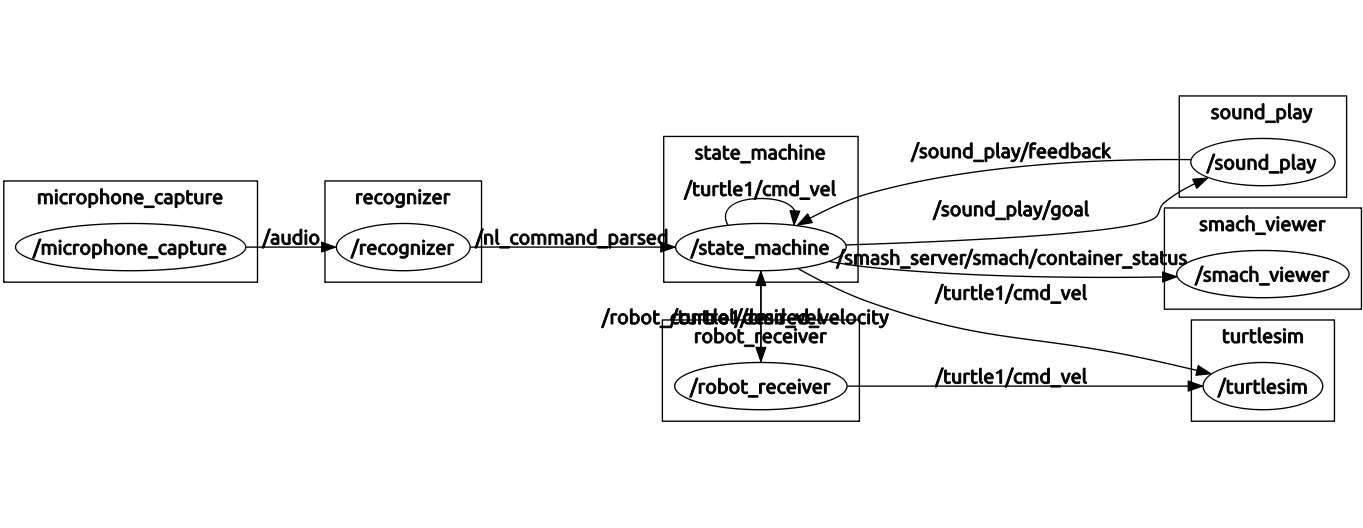
\includegraphics[width=16cm]{img_SM/rqt_graph_ALL_FINAL.png}
\caption{Diagram with the nodes and topics of the program using "rqt\_graph"}
\end{figure}

\subsection{State Machines}

In order any user can dialogue with the robot we needed to develop a state machine which will create the structure of a dialogue by following the path of a discussion developed for any possibility (see Figure 6 of the State Machine of the program).

A State Machine is a machine that stores a state in which the program is at the present time. A Machine is made of many States and each state represents an action or a step to the right proceeding of the program. Each state has inputs and outputs, those links with the state create a path and we also call this paths branches in this document.

 \begin{figure}
 \center
 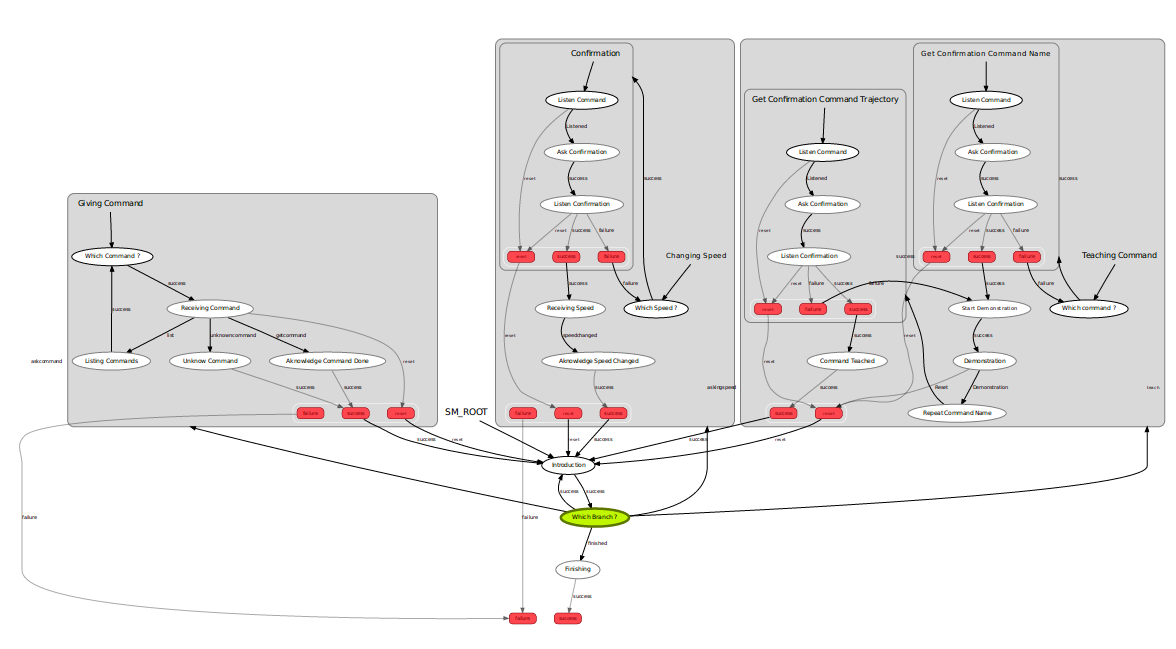
\includegraphics[width=15cm]{img_SM/StateMachine.png}
 \caption{State Machine of the program}
 \end{figure}

Regarding the specifications the robot should at least achieve three main functions. We should be able to change the speed of the robot, give a command to execute ,and teach a command. Those three functions were developed into branches. Those branches are like paths the code will have to follow to achieve what the user is asking it to do. These three branches are contained into one bigger machine called User Interface, which is the Kernel Machine. In order to simplify the code even more we also created another machine which is a Confirmation Machine, we will explain just below what it is aimed to do. Finally a State (Say State) was also independently created for the simple reason that it is a lot used throughout the project. It gives us the possibility to call this state wherever in the code.

\subsubsection{Say State}
In order to enable the robot to give speech feedback to the user we developed a state which will speak back to the user.

This state is a simple state, which is used in every machine requiring speech feedback to the user. This state publishes to the audio of the computer so then we can hear what we wanted it to say.
The main function is as explained to reproduce the sound of the string put in argument. One functionality also developed in this state is the possibility to use the user data if there is one. It will help us asking the user if the robot understood well what the user said. 
This state can then be used for everything requiring speech feedback.

\subsubsection{Kernel Machine}
The introduction is the important part where the user will be facing the possibilities the user can choose. This Introduction has been developed within the Kernel Machine.

The Kernel Machine is the central and main machine, this machine will introduce the possibility the program can do to the user by speech. This machine is composed of three states. Two Say State and one singular state (see Figure 7).

The first state cited above, the introduction one simply welcome the user and let him know what he could do with the robot. This state simply uses the sound\_play client we just learned in the first step.

The second state will listen to what the user is saying. This state was more difficult to create; in fact it has five outputs. Three of them concerned the three branches (changing speed, getting command and teaching command), one other was to quit the program and the last one was to re-branch to the introduction. 

The last state is simply a Say State which will be covered if the user want to exit the program. This state will then say "I am finished" in our case.

The general idea here was to subscribe to the topic that has transformed the speech of the user into text so then we could analyse the saying of the user. In order to make the robot act like the user wanted it to act. To do so, we had to select some keywords. For example, at the beginning we selected the keywords "speed" and "velocity" to go into the changing speed branch. Concerning the branches getting command and teaching command we choose "command" or "commanding" and "teach" or "teaching" respectively. Finally if the user said "quit", "done" or "finished" the robot will quit the program. For all the other word non-recognized we used the branch that was linked to the introduction.
In order to make the robot more interactive we developed a module, which is finding for the keywords into the text the user is saying. 

Once the base was built we could begin to develop the branches, which will allow the user to make the robot do something.  The first branch we had developed was the changing speed branch, which was the easier to begin to develop. 


 \begin{figure}
 \center
 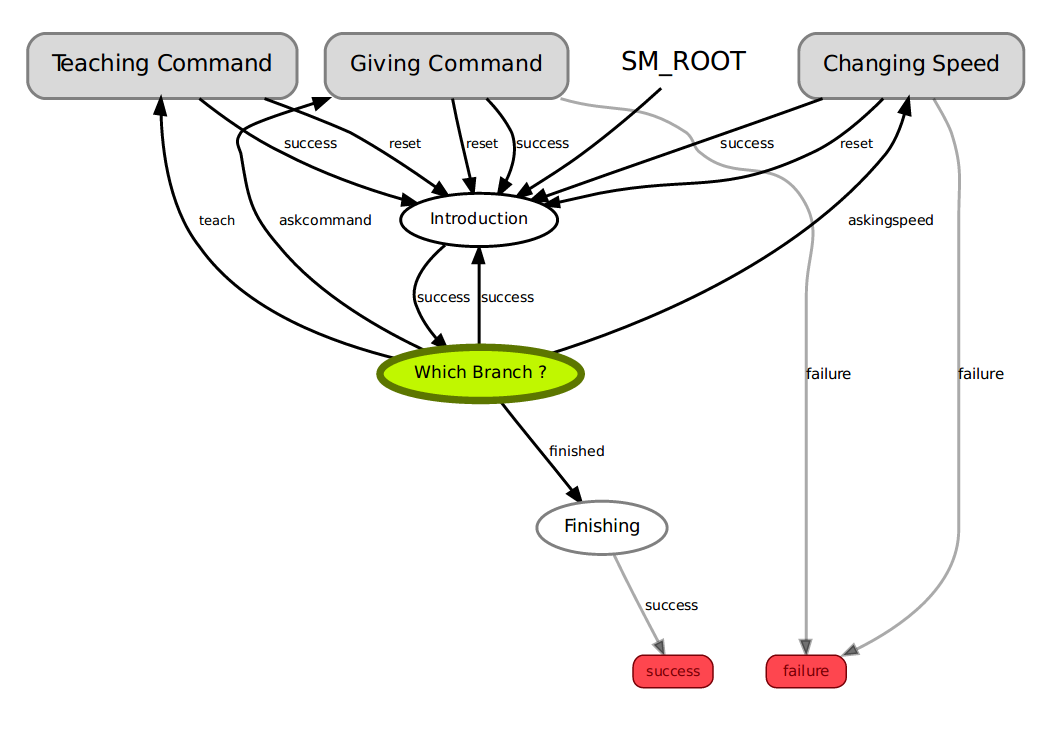
\includegraphics[width=14cm]{img_SM/KernelMachine.png}
 \caption{State Machine of the Kernel Machine}
 \end{figure}

\subsubsection{Confirmation Machine}
Sometimes the user will face some problem or will not get really well understood by the program. For this reason we developed a Confirmation Machine which will allows the user to confirm or not its saying.

This machine is aimed to ask for a confirmation and to receive an acknowledgment from the user so then the program can make sure the program understood well what the user said.

In order to take the most out of the oriented object programming we developed a machine: the Confirmation Machine which aim to ask if the word understood by the robot is the one that the user want it to understand. In fact, in order to make the user experience the best we can, we want to make sure the robot is doing what the user is asking it to do (see Figure 8).

The Confirmation Machine is made out of three states. The first and last one are considered as listener, in fact they will catch via the microphone what the user is saying and will react regarding what the user said. The second one is a simple Say State as explained above. 

The first state will simply catch what the user said by subscribing to the right topic which is the topic getting just out of the Pocketsphinx algorithm, the type of this topic is string. This data will be put as a user data in order to be accessible from another state. In fact we will need it on the state just after. There is two outputs, the regular one which goes to the second state and the one recognized by the word "reset" which will branch to the beginning of the program in case the user didn't want to go in this machine. 

The second state, which is a Say State will get the data from the state just before and as explained before in the Say State part will also say this data. This state is mainly to ask the user if the robot understood well what he said in the first state. An example of a sentence we could here there is: "Would you really like to teach the command \underline{dance}?" (the part underline correspond to the user data). There is only one output to the third state. 

Finally the third state will analyse what the user will respond to the question just ask in the second state. Regarding the keywords there will be three different outputs. In our case, we fixed "yes" and "right" for one which will branch to the end of the machine and get to the next state were this machine was called, "no" and "wrong" for a the second one which will branch to the state just before the call of the Confirmation Machine in order to re-ask the question and "reset" in order to get back to the beginning of the program.

 \begin{figure}
 \center
 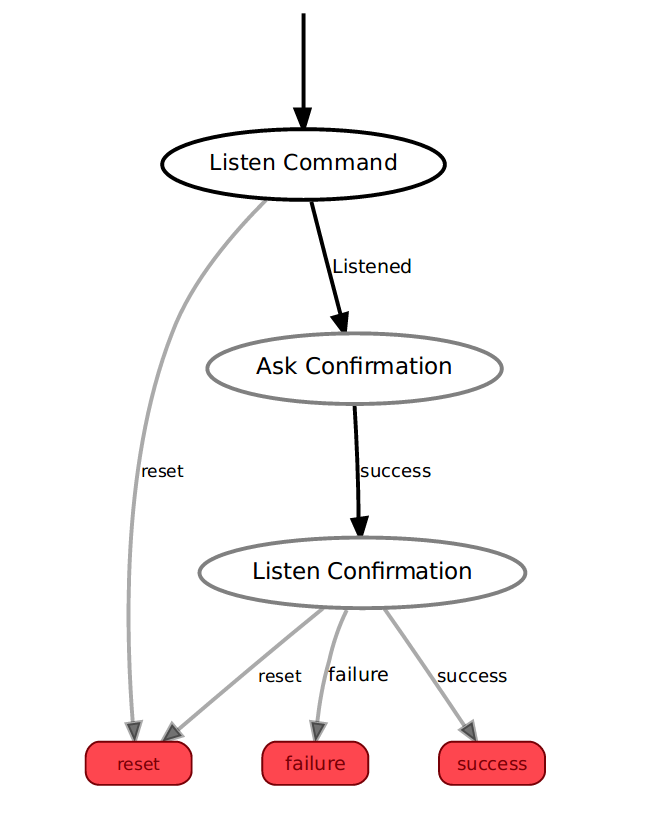
\includegraphics[width=8cm]{img_SM/ConfirmationMachine.png}
 \caption{State Machine of the Confirmation Machine}
 \end{figure}

\subsubsection{Changing Speed Machine}
The user should be able to change the speed of the robot and in order to stick to a good dialogue the user will want to hear a feedback if the speed was implemented. The user also want the possibility to correct its saying if it was misunderstood by the program.

This machine can be used to change the speed of the robot and is composed of one machine and some states: the Confirmation Machine, two Say State and one singular state (see Figure 9). 

First the machine will begin with a simple Say State, which will asks the user at which speed he wants it to move. This first state has only one outcome, which will be linked to the input of the Confirmation Machine.

The Confirmation Machine will gets in its first state the value of the speed the user wants the robot to go at. The second state will asks for acknowledgement of its understanding. The third will listen if it was well understood or not as explained in the paragraph just above. 

Once the user gets understood with the right speed by the robot it will be linked to the next state. This state serves as a converter and as a publisher. In fact the current type of the speed given by the user is string as far as we know that the Pocketsphinx algorithm will gives us strings and robots are mainly using numbers so we had to convert the strings into numbers. Once this part done we will have to publish the number corresponding of the speed given by the user to the robot converter. This state has only one output.

The final state of this machine is a simple Say State that will acknowledge to the user that the speed is changed.

 \begin{figure}
 \center
 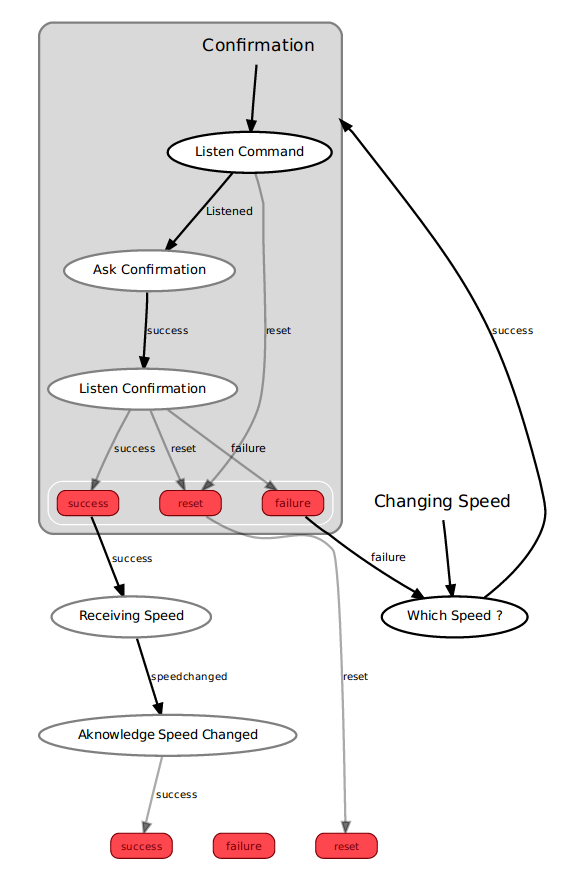
\includegraphics[width=10cm]{img_SM/ChangingSpeedBranch.png}
 \caption{State Machine of the Changing Speed Machine}
 \end{figure}

\subsubsection{Giving Command Machine}
The user should be able to give a command to execute to the robot. For this the robot needs to know all the available commands so then the user can directly pick one command from this dictionary. If the user doesn't remember all the available commands, the user should be able to access this dictionary.

This machine can be used to give a command to execute to the robot and is composed of five states four Say State and one singular (see Figure 10).

First a Say State will asks the user which command he wants it to execute. This state only has one outcome, which is linked to the second state.

The second state will be the listener; it will listen to what the user wants the robot to execute. In order to listen to what the user is saying this state is subscribing at the right topic, which is the topic getting just out of the Pocketsphinx algorithm. This state is also composed of one dictionary, which will store the possible actions the robot currently knows. Finally this state can publish the value of the command it has been taught to the robot converter. In order to treat as well as possible the wishes of the user this state has three outcomes.

The first one is linked to the third step if the command the user is saying is in the commands dictionary. This state will then acknowledge to the user that the command has been done.

The second one is called "Unknown Command" and happens if the user is waiting for more than 10 seconds or if the user says a command which is not in the dictionary. This state will branch to the output of the Giving Command Machine so then it will goes back to the beginning of the program. 

Finally the third outcome can be reached if the user is saying, in our case, the keyword "list" which will let the user knows every available commands in the current dictionary. This state is a Say State, which will use the user data to say to the user the available commands. This state will branch back the first state of the machine, which is asking which command the user wants it to do. 

 \begin{figure}
 \center
 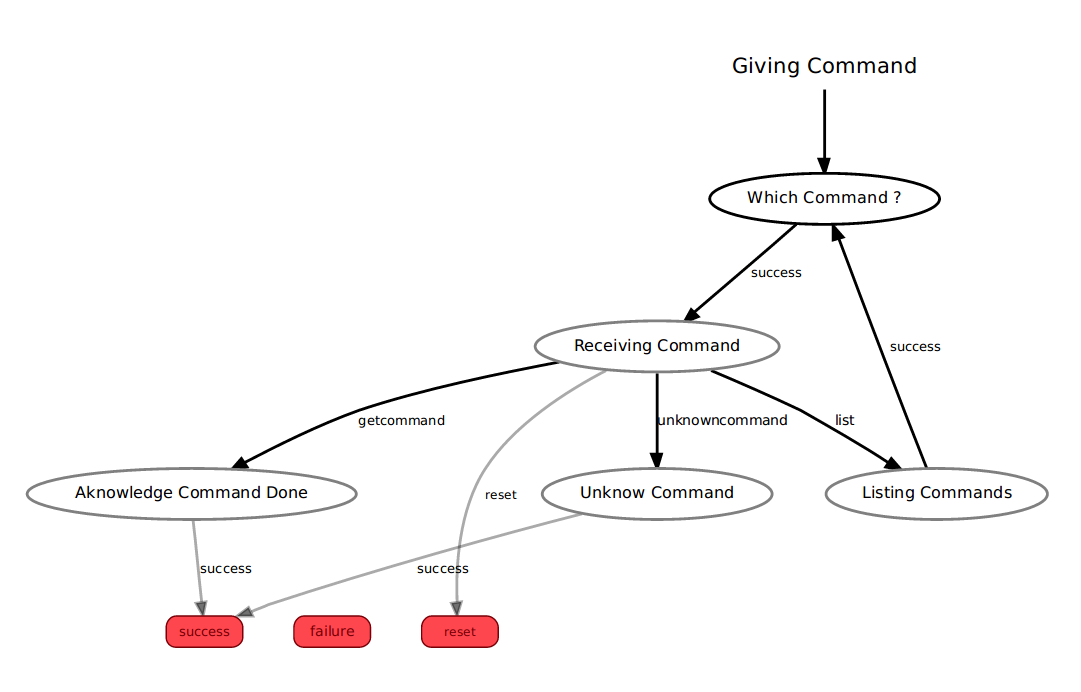
\includegraphics[width=15cm]{img_SM/GivingCommandBranch.png}
 \caption{State Machine of the Giving Command Machine}
 \end{figure}

\subsubsection{Teaching Command Machine}
The user should be able to teach a command to the robot and should be able to correct the name of the command or the trajectory the user is showing without starting from the beginning every time a mistake is made. The time of the demonstration should be clear to the user so then the user can know when to do this demonstration.

Finally the last machine developed was the Teaching Command Branch. This branch allows the user to teach a command to the robot by showing it what the user wants it to learn. This state is composed of two Confirmation Machine, four Say State and one singular (see Figure 11).

The first state is a Say State, which is asking which command the user wants to teach to the robot. This state has only one output to the second state, which is the first state of a Confirmation Machine.

At the end of the Confirmation Machine we have another Say State that gives the instructions to the user about how to record the command the user wants to teach. This state has only one output which is the demonstration state.

The demonstration state will record the movement the user is showing starting from the moment the user says: "Start" and finish recording when the user says: "Stop".
  
Then there is the third Say State which is introducing the last Confirmation Machine. This Confirmation Machine is used in order that the user could re-do the demonstration if not happy by what the user did. 

Then if the Machine is ending by a success, the dictionary of the Giving Command Branch will be implemented.

The last state will acknowledge that a new command has just been taught.

 \begin{figure}
 \center
 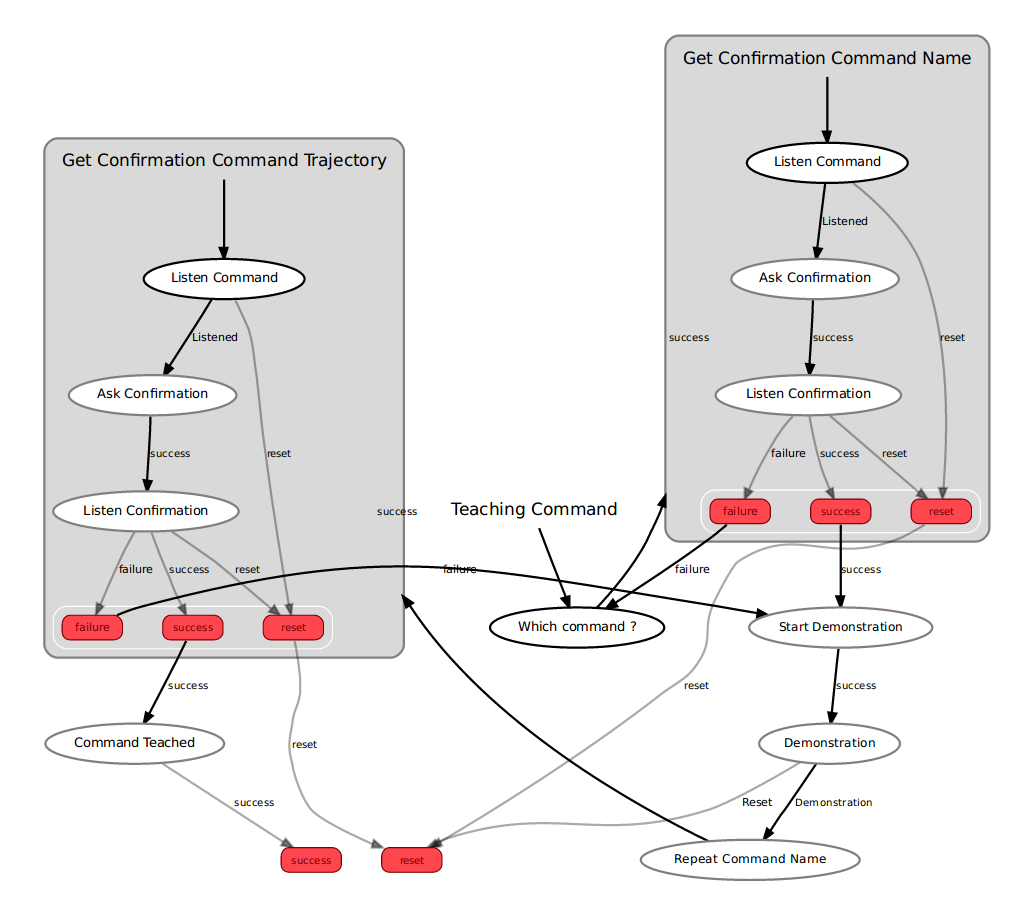
\includegraphics[width=16cm]{img_SM/TeachingCommandBranch.png}
 \caption{State Machine of the Teaching Command Machine}
 \end{figure}

\newpage
\subsubsection{Summary of major functions}
In order to sum-up the main functionality implemented in this program here is the list with a small reminder of what does each :

\begin{itemize}
  \item user-data: using this functionality of state machines allows us to access data from one state to another which will be mainly used int this program to ask for acknowledgement of the user if the robot understood well.
  \item find substring into string: this function is useful in order to let a regular discussion happens between the user and a robot. In fact this function allows to find keywords. 
  \item reset: this functionality will allow the user to get back to the beginning of the program every time the state machine is in a state called "listener" which means a state which subscribe to the output topic of the algorithm Pocketsphinx and so will listen to what the user is saying.
  \item string into numbers : in order to control the robot we need to transform the string which get out of the algorithm Pocketsphinx into numbers. This function was developed only at this effect. Once used we can publish to the converter. This function allows the user to convert only the numbers from 1 to 11. This list can be easily developed to a bigger number.
  \item time limit: this function is used in the Giving Command Branch Machine and aims to help the user if lost. In fact at the end of the state using this function, the program will branch back at the beginning.
  \item consulting the commands dictionary: again this function was developed to help the user in his experience. If the user is lost or simply forgot what he taught to the robot he can simply ask by saying the keyword "list"
  \item dynamic dictionary: this function will allows the program to implement the command dictionary every time the user teach a new command. 
  \item sound\_play wait : this function gave the possibility of waiting into the Say State until the sentence was completely read. By using an argument, we could use it or not whether it was needed in every Say State or not.
\end{itemize}



\clearpage
\section{Experiments}
In order to improve the system we decided to make two experiments. The first one was aimed to found the best keyword the algorithm will recognize the most whoever is talking with whichever accent. The comprehension of the user by the algorithm is a key factor for its success. This experiment helped us to collect the best keywords each time the user have to interact with the robot. Then we experimented at the end of the development of the program a user experience to see if it was easily usable and also gives us feedback the future work. This kind of experiments can be done again in order to check the intuitiveness of each word, or to know in which order the user would like to receive the question etc. Realizing more experiments in general would have been a good plus for the project in order to adapt the more possible our program to our consumers: everyone and not only engineers.

\subsection{Confusion Matrix}
In order to prepare this experiment some instructions were prepared for both the experimenter and the user.\\
Need for the experience: 9 persons ideally with different accents.\\
Work for each user: pronounce in a normal way a list of 24 words, 3 times. Each series will be in a different order.\\
{\itshape
\\Experimenter instructions:
\begin{enumerate}
  \item Prepare the computer to record the bagfile
  \item Launch the program (\textit{roslaunch user\_experiment robot\_voice\_control.launch})
  \item Record the topic getting in the microphone (rosbag record /audio)
  \item Let the user came in the room
  \item Give the instructions to the user (see below)
  \item End the experiment by stop recording 
  \item Give explanation why this experiment is useful
\end{enumerate}

Instructions to the user (point 5)):
\begin{itemize}
  \item Say each word one by one with a pause of 2 seconds between each word
  \item Don't talk between each word
  \item Pronounce the words normally
\end{itemize}

Concerning the words tested, we selected all the words that could be use every time the user has to say something to the robot so then we can choose the ones that fit the most for each situation. Here is the list of the 24 words:
\begin{multicols}{4}
\begin{enumerate}[label=(\Alph*)]
\item teach
\item learn
\item new
\item command
\item do
\item make
\item speed
\item velocity
\item quit
\item finished
\item finish
\item end
\item yes
\item no
\item right
\item wrong
\item true
\item false
\item list
\item reset
\item restart
\item start
\item stop
\item begin 
\item other words
\end{enumerate}
\end{multicols}
}
Once we had recorded all the audio we played them all through the Pocketsphinx algorithm in order to get what the algorithm understood out of the audio recorded. So then we can compare the difference between what should be getting out and what is really getting out. This gave us the data plotted just below with the word we fixed in vertical and the results we get in horizontal: (see Figure 12)
\begin{figure}
\center
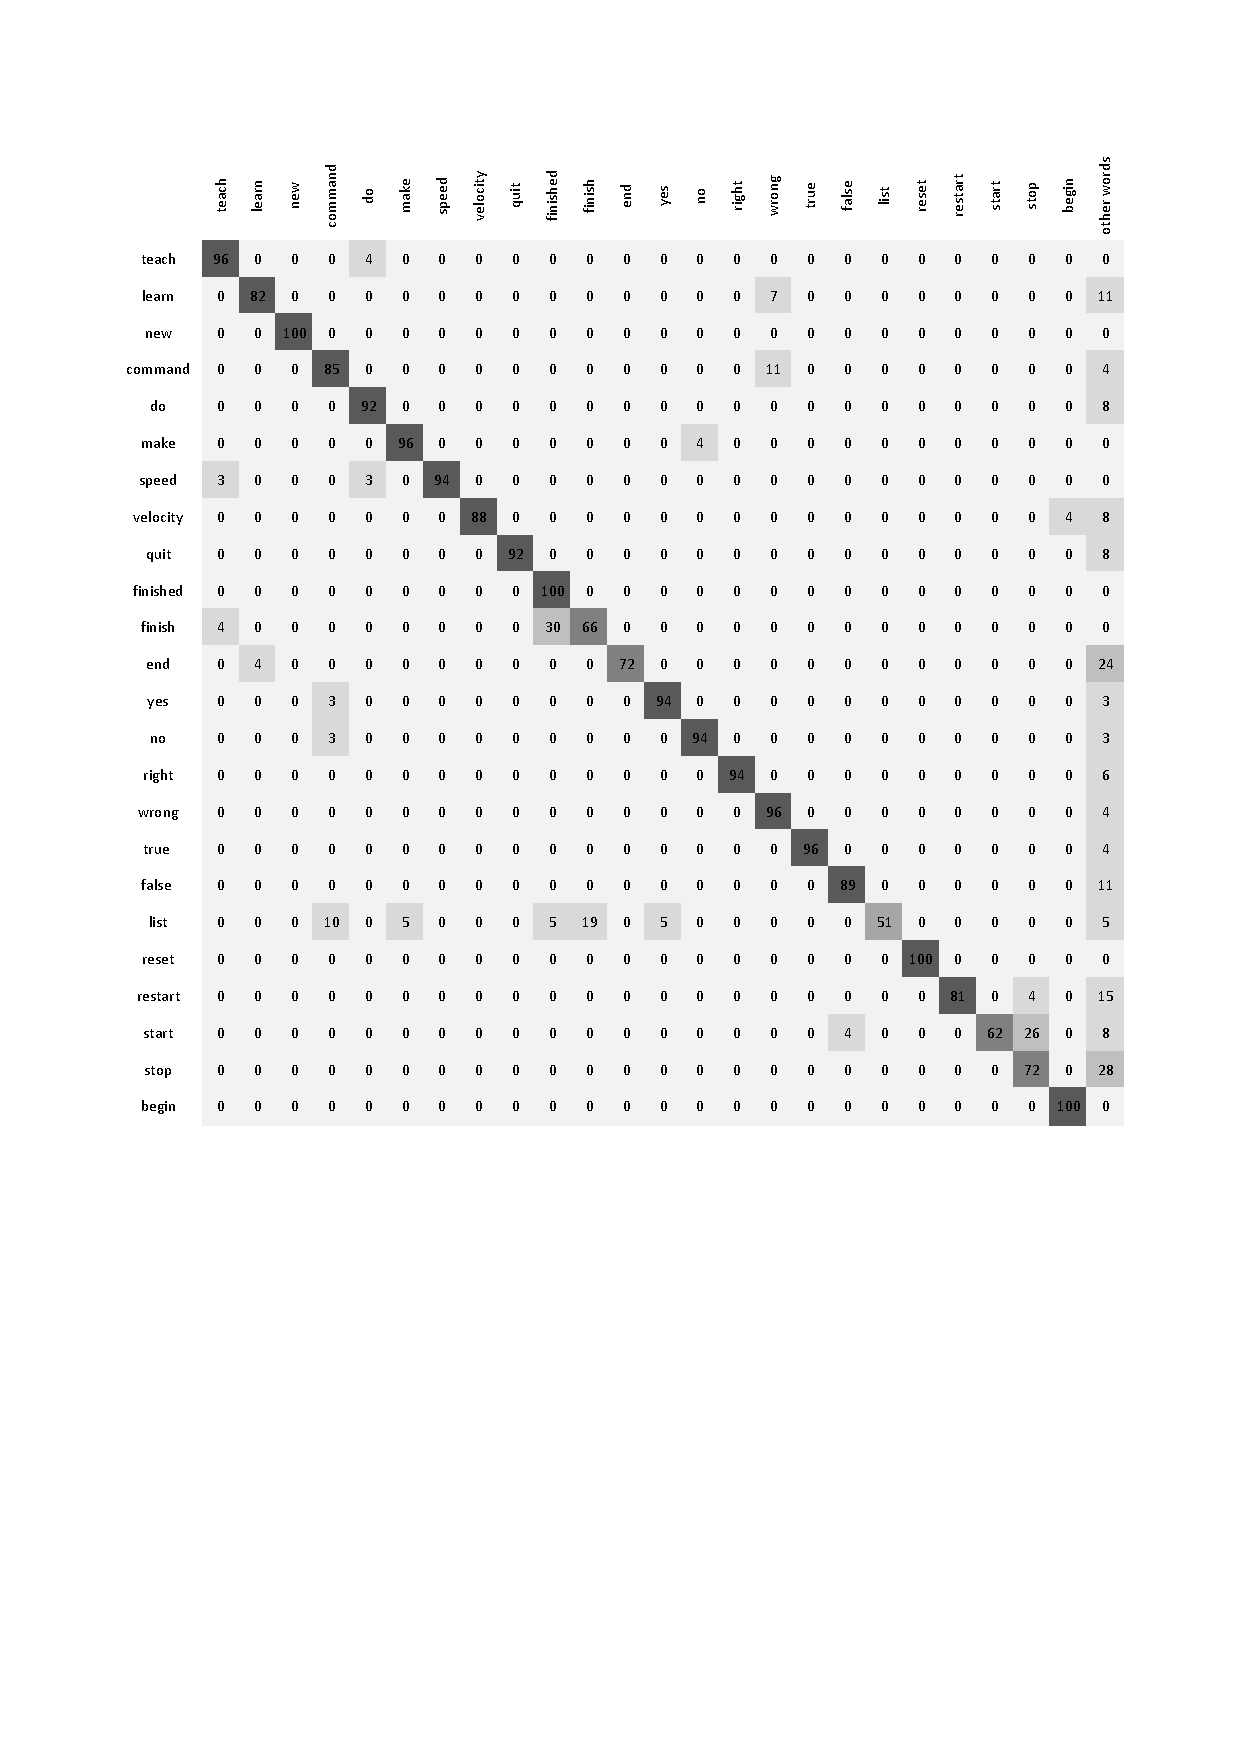
\includegraphics[width=16cm]{img/ConfusionMatrixFinal.pdf}\\
\caption{Confusion Matrix Experiment results (in percentage)}
\end{figure}

These results can let us conclude about the choice of every word for the project and here are the conclusion we made taking into consideration the results in the table and the distinctiveness of the word with all the others:
\begin{itemize}
  \item To go to the Teaching Command Machine: "Teach", "Learn" and "New"
\\We selected "Teach" and "New" since "Learn" got some confusion with some other words we cannot predict because they were in "other words".
  \item To go into the Giving Command Machine: "Command", "Do" and "Make"
\\We selected the three of them they all both got some good results. "Command" got some confusion with "Wrong", we will then remove "Wrong" from our dictionary.
  \item To go to the Changing Speed Branch: "Velocity" and "Speed"
\\We selected both words since they received some really good results.
  \item To end the program or a demonstration: "Finished", "Quit", "Finish",  "End" and "Stop"
\\We selected "Finished" and "Quit" only. The three other proposition were a lot mistaken with some other words we are using.
  \item Negation: "No", "False" and "Wrong"
\\We selected "No" and "False" since they got good results. We eliminated "Wrong" because of confusions with anterior words.
  \item Affirmation: "Yes", "Right" and "True"
\\We selected "Yes" and "True" since they got good results. We didn't select "Right" because it is the antonym of "Wrong".
  \item To access to the list of commands: "Command" and "List"
\\We selected only "Command" because "List" received some really bad results and had many confusions with words already selected.
  \item To restart: "Reset" and "Restart"
\\"Reset" got a better result than "Restart" but the results remain good so we selected both.
  \item To begin a demonstration: "Begin" and "Start"
\\We selected "Begin" and "Start". In fact in the confusion matrix we had a lot of confusion with "Stop" but we deleted it so we can assume the results will be better without "Stop".
\end{itemize}

We tried to minimize the dictionary at the maximum this is the reason we tried not put all the words with the same meaning, in fact the biggest the dictionary is, the bigger the chance a confusion between two words can be made. Minimizing the dictionary will improve the robustness of the recognition of the words said by the user.


\subsection{System Usability Scale}
The aim of this experiment was to let users who knows nothing about the project try to control the robot we developed in order to get feedback on its usability and the ways to improve. 

The user were given a paper giving the following instructions and informations:
  {\itshape
\begin{itemize}
\item Introduction:
Robot introduces itself and gives you the different opportunity you have to go through the program. It will also give you the keywords. The code will begin with an introduction and then wait in the READY STATE for you to say what you want it to do. General remark: Do not use the keyboard outside the use of teaching.

\item What you want to do? :
Once the robot introduction is done you have 4 possibilities:
\begin{itemize}
  \item Quit the program by saying the keyword � quit �
  \item Changing the speed of the branch by using the keyword � speed �
  \item Giving a command to execute to the robot by using the keyword � command � 
  \item Teach a command to the robot by using the keyword � teach �
\end{itemize}

\item Important note: 
\begin{itemize}
  \item You can reset at anytime if you are lost and want to redo it from the beginning.
  \item If the robot didn't acknowledge your saying it means that you miss-said the word: repeat yourself.
  \item You will be able to use the keyboard to teach the turtle some movements, but you won?t be able to use it any other time.
  \item Finally, every time you use the teaching branch your position will be reset at the middle of the screen. We strongly encourage you to teach everything you will need at the beginning and then try to reach the goals.
  \item When you finish the demonstration, don't forget to repeat the name of the command you are currently teaching.
\end{itemize}

\item The dictionary you have at your disposal is the following one:
Right, left, up, front, down, back, speed, � Numbers � (one to eleven), teach, start, stop, reset, velocity, wrong, right, true, false.\\


\item Experiment Explanation to the user:
\begin{enumerate}
  \item You will get 10 minutes to use the state machine and feeling comfortable with the interface.
  \item You will have to attain two goal
  	\begin{enumerate}
  	  \item The two objectives will be the following:
	  	\begin{enumerate}
		  \item First you will have to touch the right wall 
		  \item Then you will have to reach the up-left corner.
		\end{enumerate}
	\item If you are stuck and do not know what to do, you can ask for my help and I will reset the code.
	\item Every time you will teach a command to the robot, the position of the turtle will be reset.
        \end{enumerate}
  \item You will have to answer a small survey
  	\begin{enumerate}
	  \item Few questions will be asked in order to improve the project
	\end{enumerate}
\end{enumerate}

\end{itemize}
} 
For this experiment we decided to evaluate three things in addition to the completion of a System Usability Scale. The three things we evaluated were the following: 
\begin{itemize}
  \item Number of time the user required the help of the experimenter
  \item Number of time the user required information from the experimenter
  \item Number of location goals reached (the user had to reach the right border first and then the top-left corner)
\end{itemize}

Concerning the results we will analyze each user:
\begin{itemize}
  \item The first user was directly blocked at the beginning when he had to teach a command to the robot. The algorithm couldn't understand him saying "Start" to record a command. In fact during this experiment the robot had no command already taught at the beginning. Additionally to that the user felt lost once I helped him for the "Start" word because of a specificity of the code. After demonstrating the command the user wanted to teach to the robot, he had to repeat directly the name of the command he was teaching because at the beginning I didn't put a Say State at this place, again the user required my help here. Finally, instead of teaching the basics command, the user wanted to teach one command to reach each goal in one time. That wasn't the best way of doing it since the Teaching Command Machine is way longer to execute than the Giving Command Machine. Except these problems of use, the feedbacks were good. The user didn't reach the goal because of the problem with the word "Start".
  \item The second user succeeded better the experiment. The user required two times help during the experiment but reached the two goals. One of my interventions was to explain him again the problem after the demonstration and the second time was simply because he felt a bit lost since the robot didn't acknowledge something the user said. The reason is because the robot didn't understand what the user said. A simple explanation at the beginning could be to insist more on the fact that every time the user say something the user will receive a speech feedback from the robot.
\end{itemize}

Finally we fixed the problem the user encounter when teaching a command simply by adding a Say State after the demonstration which is asking the user to repeat the command he is teaching. In general the feedbacks were good and were saying that the program is easy to use and intuitive once an explanation of the program is done at the beginning by someone knowing the program.

\clearpage
\section{Discussion}
\subsection{General Discussion}
Regarding the project in general we succeeded to develop a dialogue between the robot and a user. 
By looking at the final version of the program we can say that a dialogue has been successfully created between a robot and a user. Moreover if we look at the specifications we can also say that they have been implemented despite the fact that some can be improved.

In order to make the use of the robot intuitive and easy to use without preliminary explanation we need to use the speech feedback of the robot. In fact this functionality help a lot the understanding and the step the user has to follow to control well the robot.

The structure of the dialogue has been optimized, every time the user is saying something the robot will acknowledge it. This functionality is very important, so then the user can realize if the robot understood well or not the saying of the user. Sometimes the command said by the user was even said back by the robot with the help of the global variable.

Close to the end of the semester we did the Confusion Matrix Experiment. This experiment helped us finding the best keywords we could use in our program so then the algorithm has the best chance to understand well the word whichever the accent the user has. The choice of the keywords we selected was based on the success rate of the recognition of the word by the algorithm, but also the distinctiveness with the other words in order to avoid confusion. 

In order to make this program usable on every robot we decided to develop a main structure in which everything could be the same except the converter that will convert the type we use in the State Machine (String) into the type the robot we want to use is using. 

Finally we had the chance to realize an user experience and get feedback out of it. Some of the feedback that came out were that the algorithm didn't really succeed to understand what they were saying, that led to the problem that the user felt lost because the robot weren't acknowledging anything for the reason that users were stuck in the same state, we will propose a solution for the problem in the Improvements part. The general feedback was that it was intuitive and easy to use but still needed some help from the experimenter at the beginning. \\

\subsection{Kuka Implementation}
The final step of the project was the implementation on the Kuka and it was a success. We only had to develop the converter for the Kuka in order to make it work.
We didn't stop here, in fact my project and the one of S. Ballmer were linked. S. Ballmer was developing an algorithm enabling the robot to learn movements by providing good transformed data. Assembling the two programs was the longest part of the implementation on the Kuka.
We finally made it work and we could record some video of the Kuka working.
\clearpage
\section{Future Work}
Finally this project has been developed but there is still some place for improvement. We took in consideration all the feedbacks we get from the two users who tried the program and targeted some problem we could have solved if the time was on our side. 

First of all, considering the accuracy of the Pocketsphinx algorithm and because some user couldn't get understand by it and so were blocked into one state by feeling a bit lost, we could simply let the robot repeat the state in which it is and/or the instructions every periodic amount of time (ex: 10 seconds). Moreover this function has already been developed (cf. Giving Command Machine), we should just add it in every states. More generally, some functions we developed could have been re-used a bit everywhere in the code. 

Another important thing we could have done better is to grow the user experiment (System Usability Scale) to a bigger number of subject to collect more feedback and so make a real conclusion out of it. In fact the product was designed to be use by everyone not prepared.

Concerning the Giving Command Machine, we could have simply add a functionality which could have allow the user to say command one after another without doing the full branch each time. In fact one of the feedback was also that it was kind of annoying to do the full branch for only one command. This function could have been easily developed.

As explained during the System Usability Experience, one of the user was stuck at one point because he couldn't get understand by the algorithm to teach a command. In order to face this problem we could simply use a more accurate speech-to-text algorithm which could allow us to put a lot more words without the fear of having a confusion between two similar words. It could unblocked the situation were a user is misunderstand by using the one or two keywords selected to pass a state.


\clearpage
\section{Conclusion}
To conclude this project we can say that the program is working and usable by a majority of people after a small formation on the robot. All the specifications has been completed but there is still place for improvement as we have just seen above. We can finally confirm that creating a dialogue using a state machine is an adaptable, robust and easy way to interact with robots.
\section{Aknowledgements}
I would like to thank particularly Felix Duvallet and Klas Kronander who both have been very available, present and motivative to help and support my work throughout the semester; all this work would not have been possible without them. I would like also to thanks Professor Aude Billard for the chance to do this project in the Learning Algorithms and Systems Laboratory. Finally I would like to thank all the member of the LASA Laboratory and others who took time to do some of my experiments.
\clearpage
\section{Appendix}
\subsection{Tools used for the main project}
All the tools were developed in Python.\\
Tutorial recommended: \url{https://docs.python.org/2/tutorial/}\\
The communication between each nodes of the project was done using ROS. \\
Tutorial recommended: \url{http://wiki.ros.org/fr/ROS/Tutorials}\\
\\
All the tools downloaded and developed are listed just below:\\
\\Downloaded :
\begin{itemize}
  \item Microphone capture: \textit{rosrun audio\_capture audio\_capture} \\ 
  \url{https://github.com/ros-drivers/audio\_common.git}
  \item Recognizer (speech to text): \textit{rosrun pocketsphinx recognizer.py} \\
  \url{https://github.com/cmusphinx}
  \item Sound Play: \textit{rosrun sound\_play soundplay\_node.py} \\
  \url{https://github.com/ros-drivers/audio\_common.git}
  \item Turtle Simulator: \textit{rosrun turtlesim turtlesim\_node} \\ 
  \url{https://github.com/ros/ros\_tutorials.git}
  \item Turtle Simulator Controller: \textit{rosrun turtlesim turtle\_teleop\_key} \\ 
  \url{https://github.com/ros/ros\_tutorials.git}
  \item State viewer (Smach): \textit{rosrun smach\_viewer smach\_viewer.py} 
  \item Rqt\_graph 
\end{itemize}
\hfill \\
Developped:
\begin{itemize}
  \item State Machine (Python)
  	\begin{itemize}
  		\item branch\_teachingcommand.py
  		\item branch\_gettingcommand.py
  		\item branch\_changingspeed.py
  		\item ConfirmationMachine.py
  		\item interactive\_demo.py
  		\item say\_state.py 
  	\end{itemize}
  \item Robot receiver or Converter (Python)
  	\begin{itemize}
  		\item robot\_receiver.py (for the turtle simulator)
  	\end{itemize}
  \item Nosetests
  	\begin{itemize}
  		\item test\_command\_in\_dictionnary.py
  		\item test\_string\_to\_number.py 
  	\end{itemize}
  \item Launch files
  	\begin{itemize}
  		\item pc\_interactive\_demo.launch 
  	\end{itemize}
  \item Dictionary   
  	\begin{itemize}
  		\item robot\_control.corpus 
		\item robot\_control.lm \linebreak generated by \url{http://www.speech.cs.cmu.edu/tools/lmtool-new.html} from the robot\_control.corpus file
		\item robot\_control.dic \linebreak generated by \url{http://www.speech.cs.cmu.edu/tools/lmtool-new.html} from the robot\_control.corpus file
  	\end{itemize}

\end{itemize}
\hfill \\
All of the project is available here : \url{https://github.com/epfl-lasa/nl-dynamics.git}.





\clearpage
%%%%%\begin{thebibliography}{1}

\bibitem{books} Carl Edward Rasmussen and Christopher K. I. Williams, the MIT Press {\em Gaussian Processes for Machine Learning} \url{http://www.gaussianprocess.org/gpml/} 2006.
\bibitem{documentation} ROS documentation, Open source Robotics Foundation \url{http://wiki.ros.org/}.
\bibitem{documentation} Fourier series interpolation for \autoref{equ_fourier}, Wikipedia \url{https://en.wikipedia.org/wiki/Trigonometric_interpolation}.
\bibitem{article} Cyril Schmitt {\em Simplifying user/robot interface by using speech commands}, EPFL, 2016.
\bibitem{article} Klas Kronander, {\em Gaussian Process Regression on Curves}, Technical paper, EPFL, 2016.
\bibitem{documentation} Sky McKinley and Megan Levine, {\em Cubic Spline Interpolation}, \url{http://web.archive.org/web/20090408054627/http://online.redwoods.cc.ca.us/instruct/darnold/laproj/Fall98/SkyMeg/Proj.PDF}

\end{thebibliography}

\end{document}